\documentclass[twoside,colorback,accentcolor=tud4c,11pt]{tudreport}
\usepackage{ngerman}
\usepackage[utf8]{inputenc} 
\usepackage[T1]{fontenc}
\usepackage{siunitx}
\usepackage{hyperref}
\usepackage{units}
\usepackage{upgreek}
\usepackage{biblatex}
\usepackage{graphicx}
\usepackage{float}
\usepackage{subfigure}
\usepackage[figure]{hypcap}
\usepackage{amsmath}
\usepackage{cancel}
\usepackage{braket}

\title{Laserdioden-gepumpter Nd:YAG-Laser und Frequenzverdopplung 4.6}
\subtitle{	\begin{tabular}{p{8cm}ll}
Benedikt Paul Schallmo   &   Dominik Pfeiffer \\ Matrikelnummer: 2686286  &   Matrikelnummer: 2913632       \\ email: \textaccent{ benediktschallmo@yahoo.de} & email: \textaccent{dominik@diepfeiffers.de}  
			\end{tabular} }
\subsubtitle{ \\Versuchsbetreuung : Dr. Matthias Sinther \\ Datum der Durchführung: 22.05.2027 \\ Abgabetermin: 12.06.2017    }
\institution{Institut für Angewandte Physik}
\sponsor{Hiermit erklären wir, dass wir die vorliegende Arbeit bzw. Leistung eigenständig, ohne fremde Hilfe und nur unter Verwendung der angegebenen Hilfsmittel angefertigt haben. Alle übernommenen Textstellen aus der Literatur beziehungsweise dem Internet sind als solche kenntlich gemacht. Diese Arbeit hat in gleicher oder ähnlicher Form noch keiner Prüfungsbehörde vorgelegen. \\\\ 
\begin{tabular}{lp{2em}lp{2em}l}
 \hspace{4cm}   && \hspace{4cm}  && \hspace{4cm}
 \\\cline{1-1}\cline{3-3}\cline{5-5}
 Ort, Datum     && Benedikt Schallmo && Dominik Pfeiffer
\end{tabular}  }


\dedication{}
\lowertitleback{}
\listfiles
    
\begin{document}

\maketitle 

\tableofcontents


\chapter{Einleitung und Ziel des Versuchs}
Während dem Versuch sollen einige physikalischen Eigenschaften eines Halbleiterlasers und eines Festkörperlasers untersucht werden. Zunächst wird hierfür der ideale Absorptionspunkt des Nd:YAG-Kristalls bestimmt werden, um möglichst hohe Leistungen zu erreichen. Die optimalen Einstellungen des Pumplasers sind der Ausgangspunkt, um die Arbeitsgrade aufzunehmen. Danach wird der Halbleiterlaser, der zum Pumpen des Nd:YAG-Kristalls verwendet wird, bezüglich seiner Effizienz näher betrachtet und dessen Kennlinie bezüglich Licht-/Pumpleistung aufgenommen aufgenommen. Anschließend wird der durch diesen Halbleiterlaser gepumpte Nd:YAG-Laser näher untersucht und die optimalen Arbeitskonfigurationen herausgearbeitet werden, um eine möglichst hohe Effizienz zu erreichen. Der so erzeugte Laser soll im Anschluss mittels eines KTP-Kristalls Frequenzverdopplung erzeugen. Dabei sollen einige Kenngrößen dieser, wie die Konversionseffizienz, bestimmt werden. Als letztes wird der so erzeugt Strahl bei 532 nm mit einem herkömmlichen käuflich erwerblichen Laserpointer bezüglich der Leistungseffizienz verglichen werden. 
\chapter{Physikalische Grundlagen}
In folgendem Abschnitt sollen die zur Durchführung des Versuches notwendigen physikalischen Grundlagen kurz erläutert werden. Hierzu zählen vor Allem die Prozesse in Lasern als auch in der nichtlineare Optik.
\section{Grundlagen Laser}
\subsection{Laser allgemein}
Das Akronym  \textbf{LASER} steht für "'\textbf{L}ight \textbf{A}mplification by \textbf{S}timulated \textbf{E}mission of \textbf{R}adiation"`, zu deutsch: "'Lichtverstärkung durch induzierte Emission von Strahlung"` und weist bereits auf das Funktionsprinzip des Lasers hin. Durch die Absorption von Energie aus Stößen mit anderen Atomen oder elektromagnetischer Strahlung können in Atomen Elektronen auf höhere Energieniveaus gehoben werden. Durch den Übergang in ihren Grundzustand wird die Energiedifferenz der Niveaus in der Form elektromagnetischer Strahlung freigesetzt. Bei freien Atomen geschieht dies spontan und isotrop in den Raum, wobei sowohl Phase als auch Polarität des ausgesendeten Photons zufällig sind.\\
Das Konzept der stimulierten Emission wurde zuerst von A. Einstein beschrieben, ca. 44 Jahre vor der Entwicklung des ersten Lasers (1960). Hierbei wird ein angeregtes Atom in ein geeignet gewähltes elektromagnetisches Strahlungsfeld eingebracht und so zur Emission eines dem stimulierenden Photon in Phase und Polarität übereinstimmenden Photons gebracht. Um nun über diesen Prozess das Strahlungsfeld zu verstärken, muss eine s.g. Besetzungsinversion erreicht werden. Damit ist gemeint, dass sich mehr Atome im angeregten Zustand befinden müssen als im Grundzustand. Nach der Stefan-Boltzman-Verteilung ist aber der energetisch niedrigere Grundzustand im thermischen Gleichgewicht überwiegend besetzt und das Strahlungsfeld wird nicht verstärkt oder sogar abgeschwächt. Eine Besetzungsinversion ist in einem Zwei-Niveau-System (Grundzustand und ein angeregter Zustand) so instabil, dass verwendete Laser mindesten ein Drei-Niveau-System, wenn nicht sogar ein höheres Mehr-Niveau-System aufweisen \cite{1}.\\
Der im Laufe des Versuches aufzubauende Nd:YAG-Laser arbeitet mit einem 4-Niveau-System.
\begin{figure}[H]
\centering
   	\begin{minipage}[b]{0.8\textwidth}
   	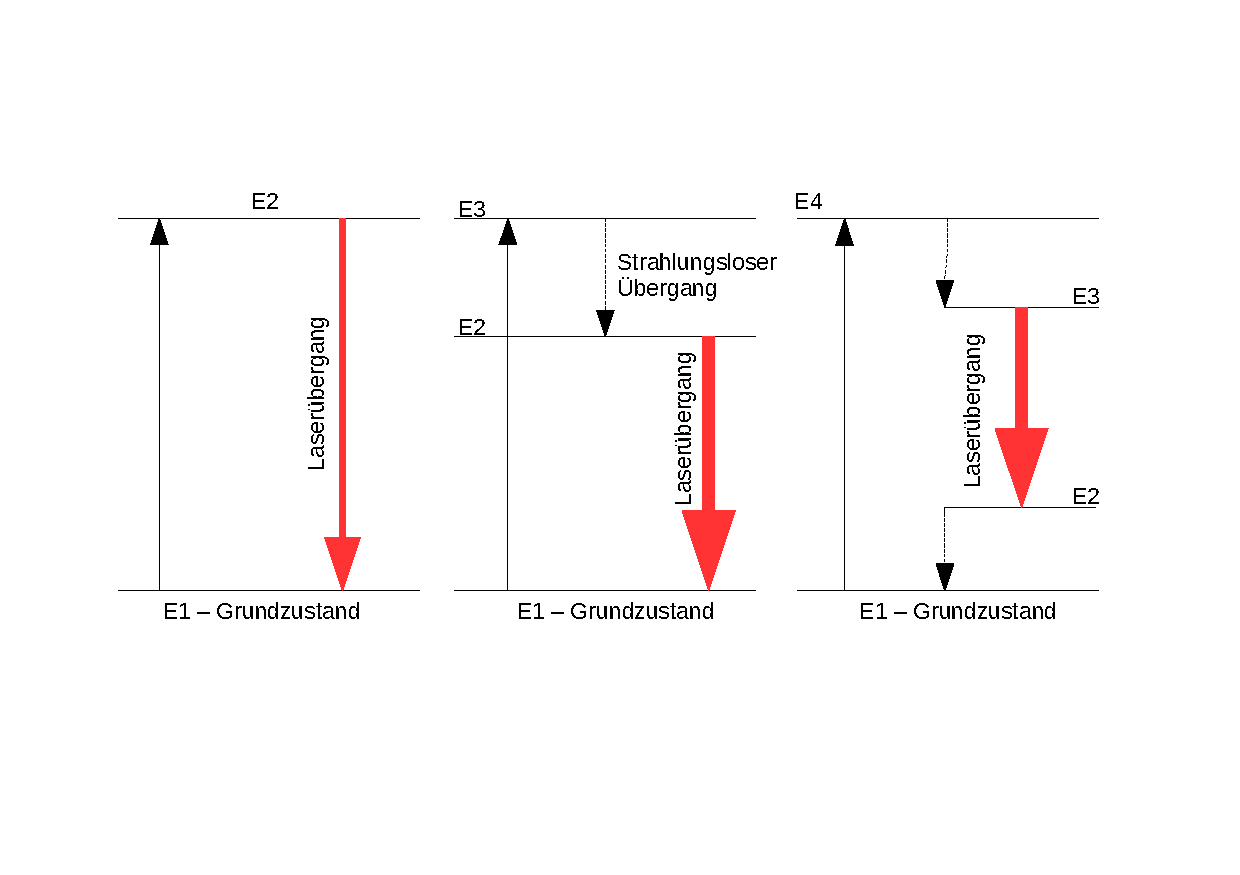
\includegraphics[width=\textwidth]{graphics/Lasersys.pdf}
  	\label{lasys}
   	\end{minipage}
\caption{Schematische Darstellung von Zwei-, Drei- und Vier-Niveau-Lasersystemen} 	
\end{figure}
\subsection{Halbleiter-Laser}
Kurz nach der Entwicklung der ersten Laser um 1960, entdeckte man auch in Halbleiterdioden Lasertätigkeit. Zunächst konnten Halbleiterlaser jedoch nur gepulst und bei geringen Temperaturen von $T<100\,\si{K}$ betrieben werden. Ab ca. 1970 konnte ein kontinuierlicher Betrieb bei Raumtemperaturen realisiert werden. Heutzutage sind Laserdioden aus dem alltäglichen Leben kaum noch wegzudenken. Sie finden in Druckern, BluRay-Playern oder Laserpointern sowie in der Medizin flächendeckend Einsatz.\\
Halbleiterlaser (HL-Laser) bestehen in der Regel aus III/V- und II/VI-Halbleitern und deren Legierungen, wobei die Römische Zahl die Hauptgruppe der Komponenten bezeichnet. Der in diesem Versuch verwendetet HL-Laser besteht aus GaAs/AlGaAs (Galliumarsenid/Alluminiumgalliumarsenid) in einer sg. Doppelheterostruktur \ref{dophet}. Der schematische Aufbau der Laserdiode ist in \ref{diau} zu sehen:
\begin{figure}[H]
\centering
   	\begin{minipage}[b]{0.6\textwidth}
   	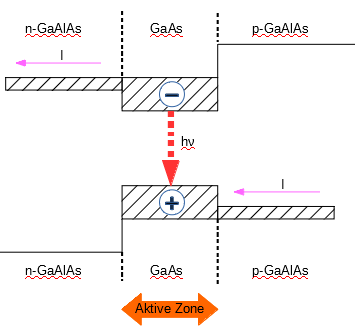
\includegraphics[width=\textwidth]{graphics/doppelhetero.pdf}
  	\label{dophet}
  	\caption{Doppelhetero-Struktur}
   	\end{minipage}
\end{figure}
\begin{figure}[H]
\centering
   	\begin{minipage}[b]{0.6\textwidth}
   	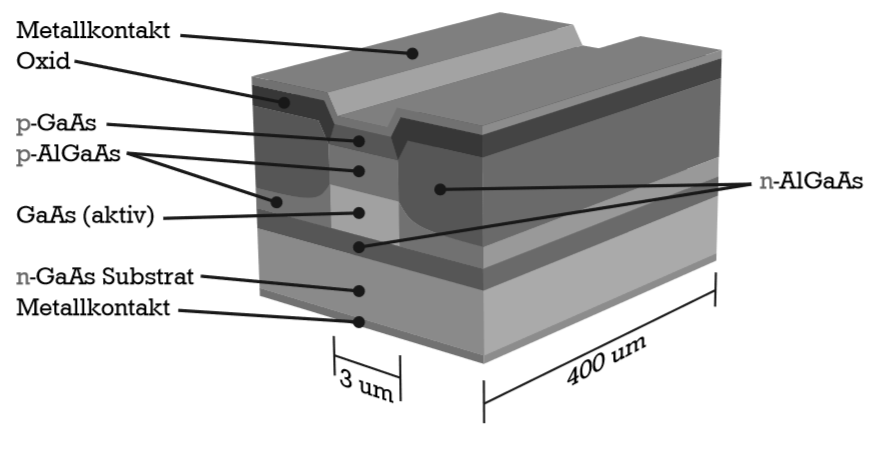
\includegraphics[width=\textwidth]{graphics/diodaufb.PNG}
  	\label{diau}
   	\end{minipage}
\caption{Aufbau der Laserdiode\cite{2}} 	
\end{figure}
Die Besonderheit von Halbleiterlasern liegt darin, dass Aufgrund der dotierten (gewollt verunreinigten) Kristallstruktur die Energieniveaus nicht mehr in diskreter Form, sondern in quasi-kontinuierlichen Form vorliegen. In einer Halbleiterdiode werden ein p- und ein n-Dotiertes Material in Kontakt gebracht. Im so entstehenden p-n-Übergang findet der eigentliche Lasertätigkeit statt. Um die Laserbedingung, also eine Besetzungsinversion zwischen Leitungs- und Valenzband zu erreichen müssen die Energieintervalle der Bänder je zu mehr als $50\%$ mit Elektronen bzw. Löchern besetzt sein. Obwohl sich die Elektronen/Löcher innerhalb des jeweiligen Bandes zwar im thermischen Gleichgewicht befinden, gilt dies mitnichten für den Halbleiter als Ganzes. Über die Quasi-Fermi-Statistik lässt sich die Besetzungswahrscheinlichkeit f(W) der Energiezustände innerhalb der Bänder beschreiben:
\begin{equation}
f(W)=\frac{1}{1+\exp\left(W-W_{L,V}\right)/ (k_{b}T)}
\end{equation}
wobei $W_{L,V}$ die Quasi-Fermienergien des betrachteten Bandes ist. Damit ergibt sich die s.g. Bernard-Duraffourg'sche Laserbedingung zu $W_{g}<h\nu <W_{L}-W_{V}$. Bei einem HL-Laser wie dem hier verwendeten erreicht man die Besetzungsinversion über das Anlegen einer Spannung in Durchlassrichtung der Diode und den daraus resultierenden Strom. \\
Um mehr stimulierte als spontane Emission zu erzwingen, muss wie bei jedem Laser ein Resonator Teil des Aufbaus sein. Bei HL-Lasern erreicht man dies, indem der Kristall entlang einer bestimmten Achse spaltet. Aufgrund des hohen Brechungsindexes des Kristalles gegenüber der Luft erzielt man so bereits eine Reflektivität von knapp 30\%, was ausreicht um Lasertätigkeit zu ermöglichen. Um das Laserlicht in bestimmte Richtungen zu führen, bettet man das aktive Medium (GaAs), in der die Rekombination von Elektronen und Löchern stattfinden soll, oftmals in andere Materialien mit niedrigerem Brechungsindex und größerer Bandlücke (AlGaAs) ein. So kann die Effizienz der Laserdioden gesteigert werden.\\
HL-Laser haben gegenüber anderen Lasersystemen einige Besonderheiten:
\begin{itemize}
\item Größe: HL-Laser lassen sich sehr kompakt bauen und passen somit auf kleinsten Raum, was vor allem bei einer Anwendung in der Technik von großem Vorteil ist.
\item Effizienz: Laserdioden erreichen mittlerweile Effizienzgarde von bis zu 70\% und sind somit deutlich effizienter als z.B. ein He-Ne-Laser.
\item Durchstimmbarkeit: Dieser Punkt ist Vor- und Nachteil zugleich, denn die emittierte Wellenlänge der Laserdiode ist empfindlich von den Faktoren Temperatur und Pumpstrom Abhängig. Für die im Versuch verwendete Diode gelten die Abhängigkeiten: $0,25\,\si{nm}/\,\si{K}$ für Temperatur und $0,05\,\si{nm}/\,\si{mA}$. Dies kann genutzt werden, um wie in diesem Fall den optimalen Arbeitspunkt für das Pumpen des Nd:YAG Lasers zu finden, kann aber bei einer gewünschten Stabilität des Lasers auch zu Problemen führen, wenn eine Temperaturkonstanz nicht ausreichend gewährleistet ist.
\item Kosten: Die Herstellungskosten von Halbleiterbauteilen wie Laserdioden belaufen sich auf einen Bruchteil von anderen Lasersystemen.
\end{itemize}\cite{1,3}
\subsection{Nd:YAG-Laser}
Der Nd:YAG Laser zählt zu den Festkörperlasern. In den Wirtskristall Yttrium-Aluminium-Granat $(Y_{3}Al_{5}O_{12})$ werden Neodym Störstellen eingebracht, es handelt sich also um einen Neodym-dotierten YAG-Kristall. Er findet weit verbreitet Anwendung wie zum Beispiel in der Technik zum Schweißen von Werkstücken oder in der Medizin bei der Behandlung von Nierensteinen. Das Energiespektrum des Lasers ist in Abbildung\ref{ndschem} zu sehen:
\begin{figure}[H]
\centering
   	\begin{minipage}[b]{0.6\textwidth}
   	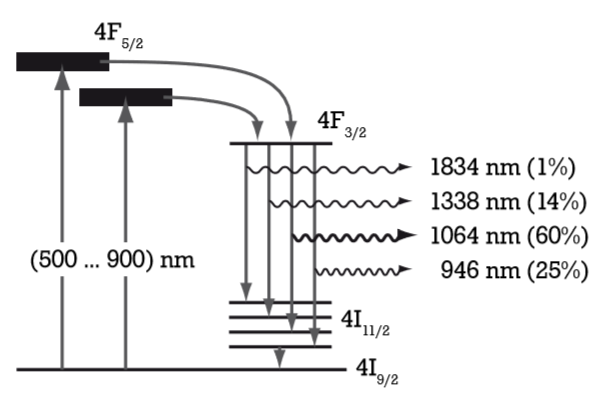
\includegraphics[width=\textwidth]{graphics/ndyagschem.PNG}
  	\label{ndschem}
   	\end{minipage}
\caption{Energienivauschema des Nd:YAG-Laser \cite{2}} 	
\end{figure}
Im Versuch wird eine Laserdiode zum optischen Pumpen des Nd:YAG Kristalls verwendet. Gepumpt wird der Laser aus dem $4I_{9/2}$ in die $4F_{6/2}$ Niveaus über Photonen mit einer Wellenlänge von \\ $500\,\si{nm}<\lambda<900\,\si{nm}$, wobei folgende Wellenlängen mit hoher Effizienz gepumpt werden können:
\begin{align}
\lambda_{1}&=804,4\,\si{nm}\\
\lambda_{2}&=808,4\,\si{nm}\\
\lambda_{3}&=812,9\,\si{nm}\\
\lambda_{4}&=817,3\,\si{nm}\\
\end{align}
In diesem Bereich liegt auch die Emission des zum Pumpen verwendeten Diodenlasers, weshalb eine Kombination der beiden mit einer hohen Gesamteffizienz betrieben werden kann.\\
Von den oberen Pumpniveaus gehen die Elektronen nach einer kurzen Lebensdauer strahlungslos in den $4F_{3/2}$, das obere Laserniveau über. Dieser Zustand ist metastabil und besitzt aufgrund der verbotenen elektrischen Dipolstrahlung eine Lebensdauer von $240\,\si{\mu s}$. Vom oberen Lasernivau gibt es nun 4 Übergänge in das aufgespaltene untere Laserniveau, von denen vor allem der zu 60\% vorkommende Übergang in das $4I_{11/2}$ Niveau mit einer Wellenlänge von $\lambda=1064\,\si{nm}$ interessant ist. Dieser ist offensichtlich nicht im von Menschen sichtbaren Wellenlängen Bereich von $\approx 400\,\si{nm}\,-\, 800\,\si{nm}$, lässt sich aber über die Frequenzverdopplung mittels eines KTP-Kristalles in Licht der Wellenlänge $\lambda=532\,\si{nm}$ konvertieren, welche im grünen Bereich des sichtbaren Spektrums liegt (siehe Kapitel \ref{freq}). \cite{2,4,5}
\section{Nichtlineare Optik}
Phänomene der nichtlinearen Optik sind Konsequenzen der Modifikation der optischen Eigenschafte von Materialien bei der Anwesenheit von Licht. In der Regel besitzt nur Laserlicht ausreichend hohe Intensitäten, um die optischen Eigenschaften zu verändern. Die Phänomene werden als nichtlinear bezeichnet, da die Antwort auf das angelegte Feld, nichtlinear von der Intensität des Feldes abhängt. Betrachtet man die Abhängigkeit der Polarisation in der linearen konventionellen Optik, so ergibt sich, dass die Polarisation $\vec{P(t)}$ linear mit dem elektrischen Feld $\vec{E(t)}$ zusammenhängt. Die Relation ist über 
\begin{align*}
\vec{P(t)}=\varepsilon_0\chi^{(1)}\vec{E}(t)
\end{align*}
gegeben, wobei $\varepsilon_0$ die elektrische Feldkonstante bezeichnet und die Proportionalitätskonstante $\chi^{(1)}$ als elektrische Suszeptibilität bezeichnet wird. In der nichtlinearen Optik wird dieser Zusammenhang verallgemeinert und wird als Potenzreihe
\begin{align*}
\vec{P}(t)=\varepsilon_0 \left[ \chi^{(1)} \vec{E}(t) + \chi^{(2)} \vec{E}^2(t) +  \chi^{(3)}\vec{E}^3(t) + \dots \right]
\end{align*} 
dargestellt, wobei $\chi^{(2)}$ und $\chi^{(3)}$ als optische Suszeptibilitäten zweiter und dritter Ordnung bezeichnet werden. Dieser Zusammenhang, der voraussetzt, dass das Medium instantan antwortet, gilt jedoch nur unter Vernachlässigung von Absorption und Dispersion. Die Suszeptibilitäten hängen in der Regel noch von der Frequenz ab. Dabei beschreibt $\chi^{(1)}$ zum Beispiel Brechung und lineare Absorption, $\chi^{(2)}$ die Erzeugung der zweiten Harmonischen, das parametrische Mischen und die Erzeugung von Summen und Differenzfrequenzen und $\chi^{(3)}$ die Erzeugung der dritten Harmonischen, Raman- und Brillouin-Streuung und den Kerr-Effekt. \cite{2,6}


\subsection{Frequenzverdopplung}\label{freq}
Bei der Frequenzverdopplung entsteht bei der Bestrahlung bestimmter Materialien mit Licht hoher Intensität Licht mit der doppelten Frequenz. Die elektromagnetische Strahlung regt im Material die Elektronen zum Schwingen an. Die Elektronen schwingen dabei mit der gleichen Frequenz wie die einfallende Strahlung, und erzeugen somit erneut elektromagnetische Strahlung. Bei hohen Intensität werden die Elektronen weiter ausgelenkt und die Rückstellkräfte sind nicht mehr proportional zur Auslenkung. Die dielektrische Polarisation des Materials ist nicht mehr linear vom elektrischen Feld abhängig, sondern es treten Terme höherer Ordnung auf. Dies führt dazu, dass die Polarisation außer der Frequenz der einfallenden Welle $\omega$ auch höhere Harmonische $m\cdot \omega$ ($m=2,3,4,...$) enthält. Die elektrischen Dipole strahlen daher auch elektromagnetische Wellen auf höheren Harmonischen ab. Die Erzeugung der zweiten Harmonischen resultiert aus dem Teil der atomaren Antwort, die quadratisch mit der Stärke des angelegten optischen Feldes zusammenhängt. Die Frequenzverdopplung, die Erzeugung der zweiten Harmonischen, wird wird auch als SHG (second harmonic generation) bezeichnet, die Frequenzverdreifachung als THG (third harmonic generation). 
Das elektrische Feld, welches durch
\begin{align*}
\vec{E}(t)=\vec{E}\cdot\text{e}^{-i\omega t} + c.c.
\end{align*}
repräsentiert wird, fällt auf einen Kristall dessen Suszeptibilität zweiter Ordnung nicht Null ist, und erzeugt die nichtlineare Polarisation zweiter Ordnung
\begin{align*}
\vec{P}^{(2)}(t)=2\epsilon_0\chi^{(2)}EE^*+\left(\epsilon_0\chi^{(2)}E^2\text{e}^{-i2\omega t}+c.c.\right)
\end{align*} 
Die Polarisation zweiter Ordnung setzt sich aus einem Term mit Frequenz Null und einem Term mit Frequenz $2\omega$ zusammen. Der zweite Beitrag erzeugt Strahlung mit der doppelten Frequenz, wohingegen der erste Term keine elektromagnetischer Strahlung erzeugt, sondern erzeugt ein statisches elektrisches Feld im Kristall (optische Gleichrichtung).
Anschaulich werden zwei Photonen der Frequenz $\omega$ zerstört und ein Photon der Frequenz $2\omega$ wird in einem einzelnen quantenmechanischen Prozess erzeugt. Die Frequenzverdopplung kann beispielsweise genutzt werden, um die Laserstrahlung des Nd:YAG-Lasers, der im nahen Infrarotbereich bei 1064 nm arbeitet, in den sichtbaren Spektralbereich bei 532 nm zu konvertieren. Von entscheidender Bedeutung für den Prozess der Frequenzverdopplung ist die Phasenanpassung. Die ursprüngliche Wellenlänge und die erzeugte doppelte Wellenlänge müssen im Kristall den gleichen Brechungsindex besitzen, da sonst destruktive Interferenz auftritt.
\cite{2,6,7}	
\chapter{Versuchsdurchführung und Beobachtung}
Die Durchführung richtet sich nach der Reihenfolge der Anleitung und ist im groben in sechs Teile gegliedert, welche im Folgenden kurz beschrieben werden sollen. Im Laufe des Versuches wird ein diodengepumpter Festkörperlaser mit einem frequenzverdoppelten Bauteil aufgebaut, der eine Wellenlänge von $\lambda =532\,\si{nm}$ emittiert.Hierfür werden nach und nach weitere Bauteile dem Aufbau hinzugefügt. Systeme dieser Art finden heute weitreichend Anwendung wie z.B. in grünen Laserpointern. Ein solcher wird im letzten Teil des Versuches in einem Gesichtspunkt mit dem aufgebauten System verglichen.\\
Die folgende Grafik zeigt den Versuchsaufbau mit allen eingebauten Komponenten, die im Laufe des Versuches schrittweise ergänzt wurden:
\begin{figure}[H]
\centering
   	\begin{minipage}[b]{0.9\textwidth}
   	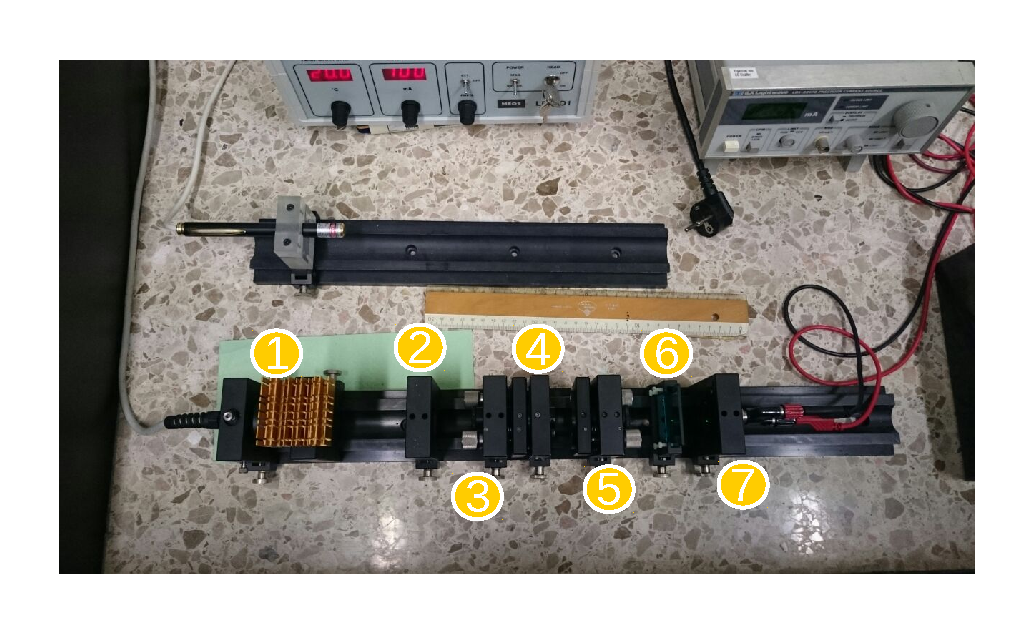
\includegraphics[width=\textwidth]{graphics/aufbau.pdf}
  	\label{vauf}
   	\end{minipage}
\caption{Versuchaufbau}	
\end{figure}
Dabei bezeichnen sind die einzelnen Komponenten:
\begin{itemize}
\item[1] Halbleiter-Laserdiode mit Vorrichtung zum ableiten der Wärme.
\item[2] Kollimator und Fokussierlinse
\item[3] Nd:YAG Kristall in einstellbarer Halterung
\item[4] KTP-Kristall zur nichtlinearen Frequenzverdopplung in einstellbarer Halterung
\item[5] Einstellbarer Spiegel für den optischen Resonator
\item[6] Halterung für den optischen Abschwächer, RG1000 oder BG39 Filter
\item[7] Photodiode zum Vermessen des Photostromes/Laserleistung
\end{itemize}
\section{Realtive Absorption des Nd:YAG}\label{v1}
Zu Beginn des Versuches soll zunächst die relative Absorption des Nd:YAG Kristalls in Abhängigkeit der Temperatur der Halbleiterdiode bestimmt werden. Der Aufbau besteht hierfür zunächst aus der Halbleiter-Laserdiode mit Quelle und Temperatursteuerung, einem Kollimator, dem Nd:YAG-Kristall, einem Abschwächer und einer Photodiode. Es werden in Abhängigkeit der Temperatur der Photodiode in einem Intervall von 10°C 40°C im Abstand von 2°C Werte des Photostromes, sowohl mit als auch ohne Nd:YAG, aufgenommen, wobei die Temperatur bei konstantem Pumpstrom so variiert wird, dass dieser maximal wird. Die Messwerte sind in Kapitel \ref{relabs} zu sehen.\\
Ziel ist es, den zum Pumpen des Nd:YAG-Kristalls optimalen Arbeitspunkt des Halbleiterlasers zu finden. Dieser ist bei einer Wellenlänge von $\lambda_{Pump}=808,4\,\si{nm}$ zu finden, diese kann jedoch nicht direkt an der Laserdiode eingestellt werden.
\section{Arbeitsgerade der Laserdiode}\label{v2}
Nachdem im ersten Teil des Versuches die für den maximalen Pumpstrom optimale Temperatur zum Pumpen bestimmt wurde, soll nun für weitere Werte des Pumpstromes die optimale Temperatur gefunden werden, um den Nd:YAG bei einer Wellenlänge von $\lambda_{Pump}=808,4\,\si{nm}$ effektiv zu Pumpen. Hierfür stellt man zunächst den maximalen Pumpstrom von $I_{Pump}=700\,\si{mA}$ und die optimale Temperatur ein und nimmt für weitere, niedrigere Werte des Pumpstromes die Temperatur auf, bei der der Photostrom maximal wird. Die Messwerte sind in Kapitel \ref{arbger} aufgetragen.
\section{Kennlinie der Laserdiode}\label{v3}
Im nächsten Schritt soll die Kennlinie der Laserdiode aufgenommen werden. Hierfür werden Wertepaare von Pumpstrom und Photostrom aufgenommen werden, wobei die Temperatur jeweils so eingestellt wird, dass man sich entlang der Arbeitsgeraden der Laserdiode bewegt.Hierfür wird der selbse Aufbau wie bisher verwendet, jedoch muss der Nd:YaG-Kristall aus dem Strahlengang entfernt werden. Über die Kennlinie der Diode lässt sich der Schwellstrom der Diode herausfinden. Die Daten zu dieser Messung sind in Kapitel \ref{kennd} angegeben.
\section{Kennlinie des Nd:YAG}\label{v4}
Um die Kennlinie des Nd:YAG-Lasers aufzunehmen geht man prinzipiell gleich vor wie zur Bestimmung der Kennlinie der Laserdiode. Hierfür wird der Nd:YAG wieder in den Strahlengang eingebaut und um einen optischen Resonator zu erhalten ein sphärischer Resonatorspiegel hinter diesen eingebaut. Des weiteren wird statt des optischen Abschwächers nun ein RG1000 Farbfilter von Schott verwendet, der für die Pumpstrahlung eine geringe Transmission von $\approx 10^{-4}$ aufweist (Messdaten siehe Kapitel \ref{kennND}).
\section{Einbau und charakterisierung des KTP}\label{v5}
Nun soll im nächsten Teil des Versuches die Wellenlänge des Nd:YAG-Lasers $\lambda_{Nd:YAG}=1064\,\si{nm}$ mittels eines nicht linearen KTP-Kristalls auf eine Wellenlänge von $\lambda_{KTP}=532\,\si{nm}$ frequenzverdoppelt werden, welche im sichtbaren grünen Spektralbereich liegt. Dafür wird dieser Kristall in den optischen Resonator zwischen den Nd:YAG-Kristall und den Resonatorspiegel eingebaut und der Spiegel so optimiert, dass der Photostrom bei maximalem Pumpstrom ebenfalls maximal wird. Des Weiteren wird der RG1000 Filter gegen einen BG39 Filter getauscht, welcher im Bereich der grünen Wellenlänge eine hohe Transmission aufweist und die Fundamentale ($\lambda_{Nd:YAG}=1064\,\si{nm}$) sowie die Pumpstrahlung ($\lambda_{Pump}=808,4\,\si{nm}$) herausfiltert. Danach wird wie bei den vorherigen Kennlinien entlang der Arbeitsgraden des Nd:YAG-Kristalls gemessen. Die zugehörigen Messdaten befinden sich in Kapitel \ref{kennktp}.
Des Weiteren wird eine Messreihe mit dem RG1000 Filter mit dem gleichen Aufbau aufgenommen, um die restliche Fundamentalleistung, die nicht im KTP-Kristall frequenzverdoppelt wurde, zu vermessen (siehe Kapitel \ref{restfund}).
\section{Kommerzieller Laserpointer}\label{v6}
Nachdem im laufe des Versuches ein System ähnlich zu denen in einem grünen Laserpointer aufgebaut und charakterisiert wurde, soll dieses nun im Bezug auf die Leitungseffizienz und restliche Fundamentalleistung verglichen werden. Hierfür wird der Laserpointer sowohl mit dem RG1000 als auch mit dem BG39 Filter vermessen. Zur Bestimmung der in den Pointer gepumpten elektrischen Leitung wird zusätzlich die Betriebsspannung und der Pumpstrom notiert.
  
     	
\chapter{Auswertung}
Da im Laufe des Versuches der grüne Laser schrittweise aufgebaut wurde, erfolgt auch die  Auswertung des Versuches in derselben Reihenfolge für jedes neue Bauteil. Zu Beginn betrachtet wir zunächst die Halbleiter GaAs-Diode, die zum optischen Pumpen des Nd:YAG-Kristalls verwendet wird.
\section{Absorptionsmessung}
Um die für das Pumpen den Nd:YAG-Kristalls bei einem maximalen Pumpstrom von $I_{P,max}=700\,\si{mA}$ optimale Wellenlänge der Halbleiterdiode zu finden, wird zunächst das Absorptionsverhalten des Nd:YAG vermessen. Da die Wellenlänge nicht direkt gemessen werden kann, nutzt man aus, dass sich bei einem konstanten Strom die Wellenlänge der Diode über die Temperatur durchstimmen lässt. Hierfür wurde wie in Kapitel \ref{v1} beschrieben vorgegangen. In Abbildung \ref{abs} ist die relative Absorption des Kristalls aufgetragen:
\begin{figure}[H]
\centering
   	\begin{minipage}[b]{0.85\textwidth}
   	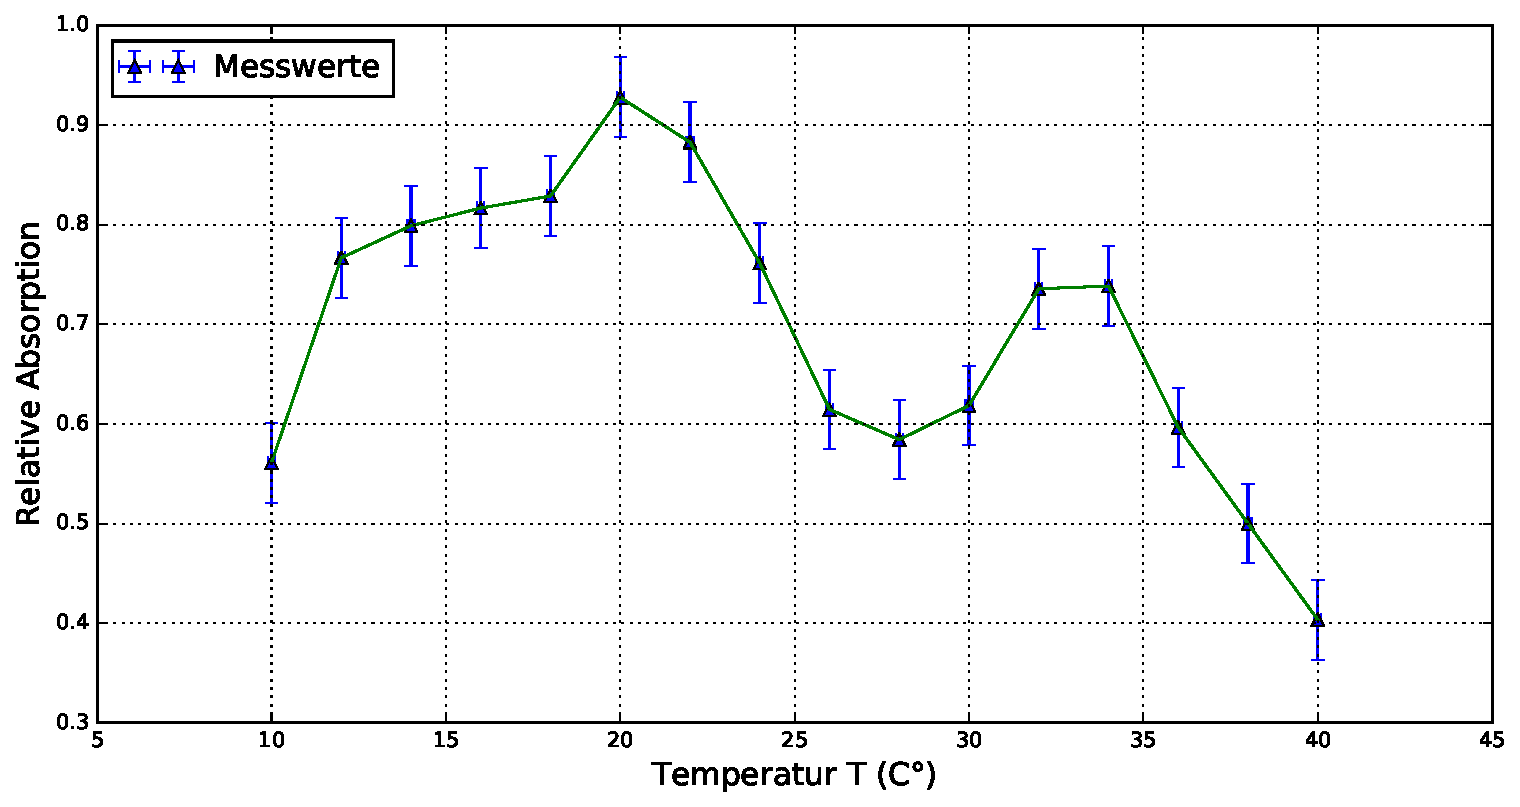
\includegraphics[width=\textwidth]{graphics/relabs_ndyag.pdf}
  	\label{abs}
   	\end{minipage}
\caption{Relative Absorption des Nd:YAG-Kristalls}	
\end{figure}
Durch einen Vergleich mit einem vorhandenen Absorptionsspektrum, bei dem die Wellenlängen angegeben waren konnte der Punkt $(I,T)=(700\,\si{mA},20\,\si{^{\circ}C})$ der optimalen Pumpwellenlänge $\lambda_{Pump}=808,4\,\si{nm}$ zugeordnet werden. Dieses Wertepaar diente auch als Ausgangspunkt für die Bestimmung der Arbeitsgeraden im nächsten Abschnitt.

\section{Halbleiterlaser}
Die im Versuch verwendete Halbleiter-Laserdiode ist eine s.g. GaAs/AlGaAs-deiode in einer Doppelheterostruktur, welche bereits in der Vorbereitung näher betrachtet wurde. Um dieses Bauteil besser zu charakterisieren betrachten wir zunächst die Kennlinie dieser Diode, also die Abhängigkeit der Lichtleistung von der elektrisch gepumpten Leistung bzw. dem Pumpstrom $I_{Pump}$. Die Kennlinie wurde wie in Kapitel \ref{v3} beschrieben bestimmt und ist in Abbildung \ref{kd} zu sehen.
\begin{figure}[H]
\centering
   	\begin{minipage}[b]{0.85\textwidth}
   	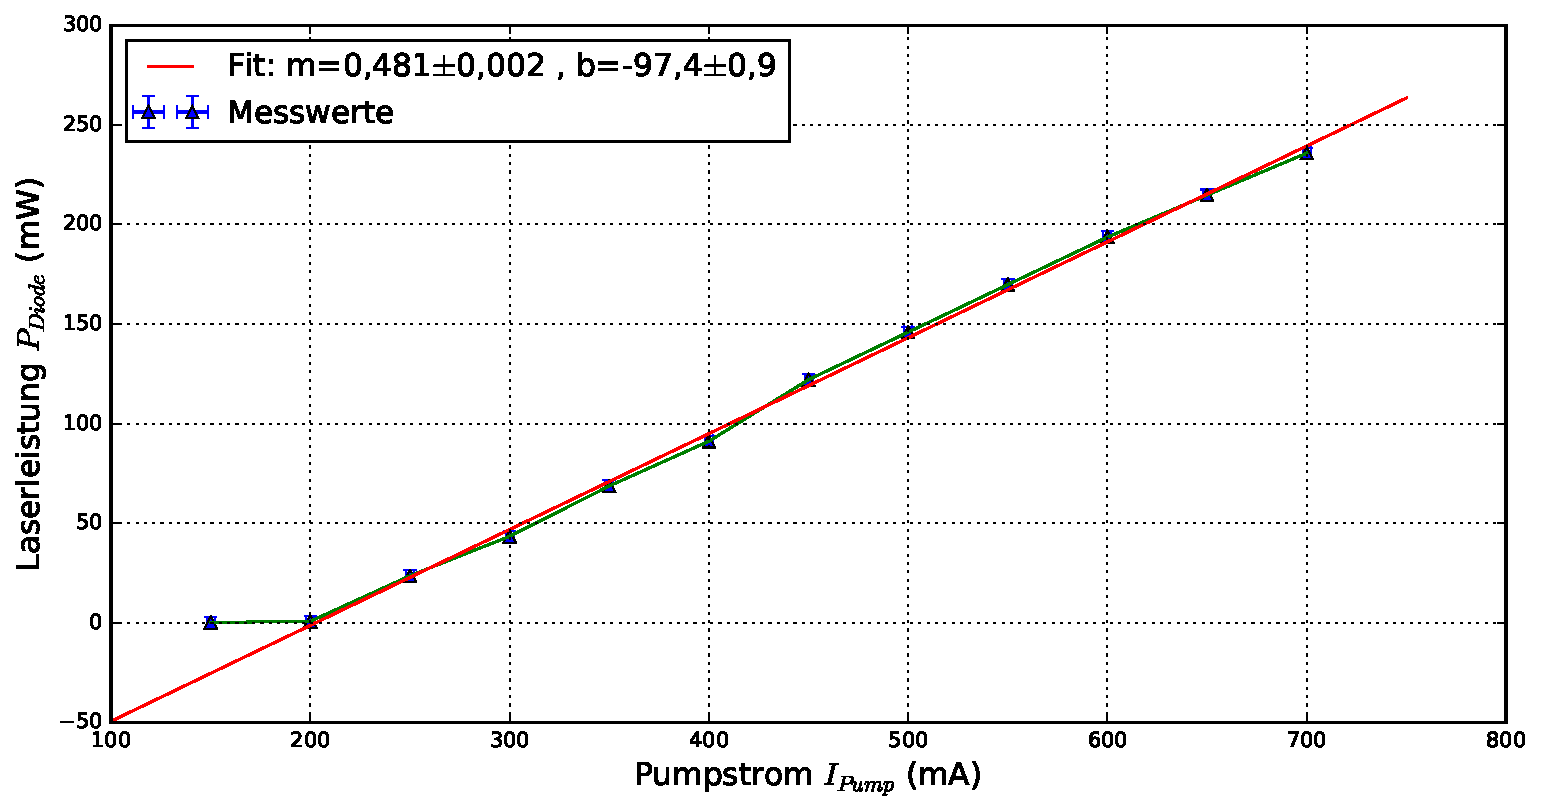
\includegraphics[width=\textwidth]{graphics/kennlinie_diode.pdf}
  	\label{kd}
   	\end{minipage}
\caption{Kennlinie der Halbleiter-Laserdiode mit Ausgleichsgerade}	
\end{figure}
An die Daten wurde mit $P_{Diode}(I_{Pump})=m\cdot I_{Pump} +b $ linear gefittet. Für den Fit ergaben sich folgende Werte:
\begin{align}
m=& (0,0481 \pm 0,002)\,\si{\frac{mW}{mA}}\\
b=& (-97,4 \pm 0,9)\,\si{mW}
\end{align}
Mithilfe dieser Fitfunktion lässt sich der Schwellstrom der Diode, also der minimal nötige Strom um Laseraktivität anzuregen bestimmen zu $I_{Schwelle}=(202,44\pm 0,80)\,\si{mA}$.\\

\begin{figure}[H]
\centering
   	\begin{minipage}[b]{0.85\textwidth}
   	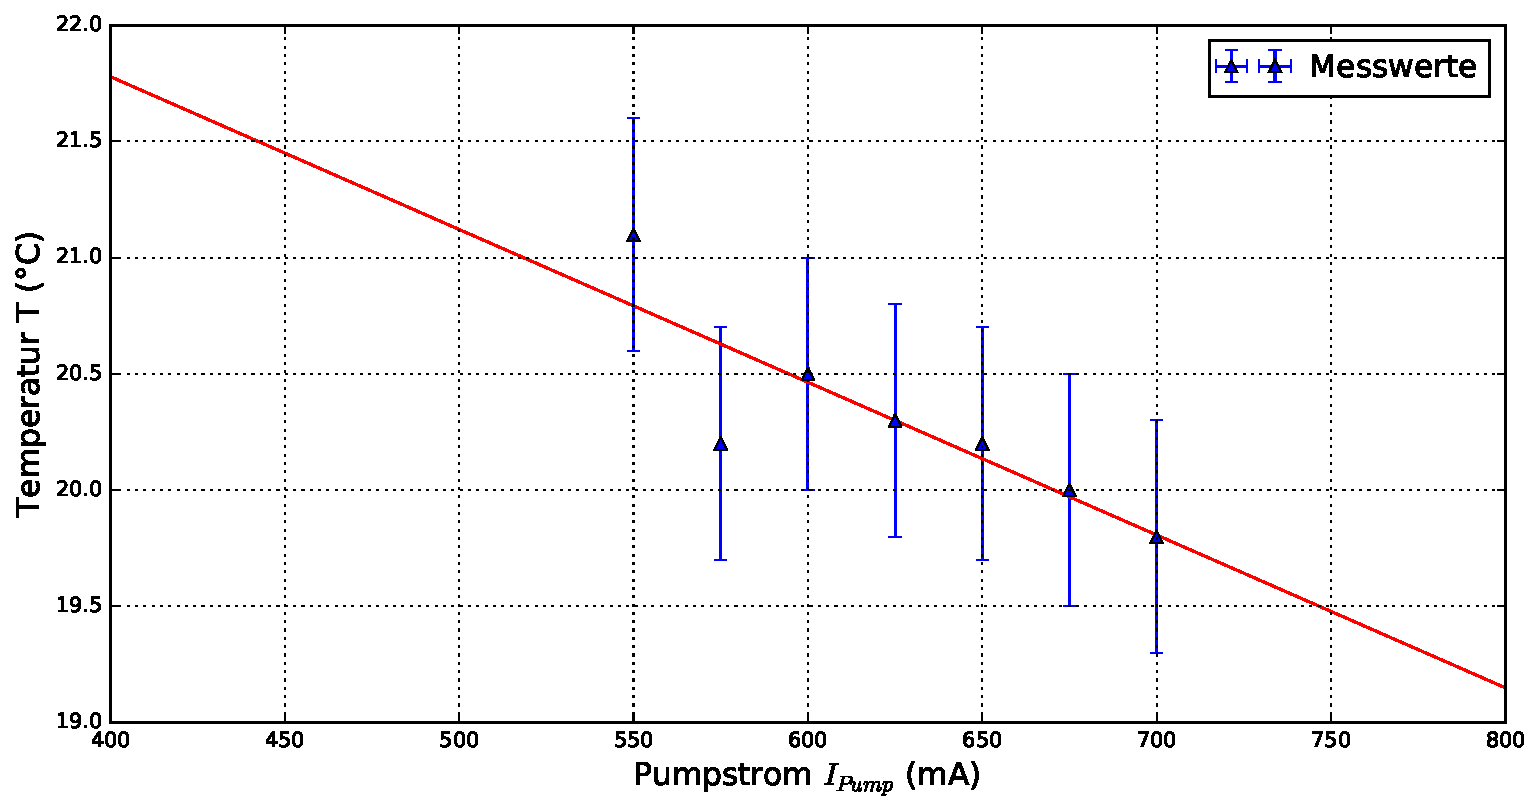
\includegraphics[width=\textwidth]{graphics/arbeitsgerade_hld.pdf}
  	\label{ad}
   	\end{minipage}
\caption{Arbeitsgerade der Halbleiter-Laserdiode mit Ausgleichsgerade}	
\end{figure}
Da Halbleiterlaser eine, in Grenzen, variable Wellenlänge haben, welche von der Temperatur und dem Pumpstrom abhängig ist und die Kennlinie für eine Wellenlänge von $\lambda\approx 808,4\,\si{nm}$ bestimmt werden sollte, ist es nötig sich entlang der für diese Wellenlänge typischen Arbeitsgeraden zu bewegen. Mithilfe dieser lässt sich eine Abhängigkeit der Temperatur vom Pumpstrom bestimmen, bei der die Wellenlänge konstant ist. Bestimmt wurde diese Arbeitsgerade wie in Kapitel \ref{v2} beschrieben und ist in Abbildung \ref{ad} dargestellt.

Die sich aus dem linearen Fit ergebenden Werte sind:
\begin{align}
m=&(-0,007 \pm 0,008)\,\si{\frac{^{\circ} C}{mA}}\\
b=&(24,4 \pm 4,7)\,\si{^{\circ} C}
\end{align}
Mithilfe dieser Arbeitsgeraden wurde die Temperatur stets so angepasst, dass die Zentralwellenlänge von $\lambda\approx 808,4\,\si{nm}$ konstant bleibt und der Nd:YAG Effizient gepumpt werden kann.\\
Als letzte, nur den Halbleiter betreffende Kenngröße soll die differentielle Quanteneffizienz $\eta$ bestimmt werden. Diese stellt das Verhältnis der Zahl der erzeugten bzw. gemessenen Photonen zu der Zahl der gepumpten Elektronen über der Laserschwelle dar. Mit der Steigung der Kennlinie der Diode $m=\dfrac{P_{Licht}}{I-I_{Schwelle}}$,sowie $h\nu=\dfrac{hc}{\lambda}$ ($\lambda=808,4\,\si{nm}$) ergibt sich:
\begin{equation}
\eta=\frac{e\cdot P_{Licht}}{h\nu (I-I_{Schwelle})}=\frac{e\cdot\lambda\cdot m}{h\cdot c}=0,314 \pm 0,001.
\end{equation}
Es werden also ca. $30\%$ aller gepumpten Elektronen in Laserphotonen umgewandelt, während die restlichen Elektronen nicht zur Lasertätigkeit im gewünschten Wellenlängenbereich beitragen.

\section{Nd:YAG-Laser}
Nachdem die Halbleiterdiode charakterisiert wurde, wird im nächsten Schritt wie in Kapitel \ref{v4} beschrieben der Nd:YAG-Kristall samt optischem Resonator in den Strahlengang eingebaut und die mit das System anhand der gemessenen Lichtleistung optimiert. Wie bereits für den Halbleiter wurde auch für das erweiterte System die Kennlinie aufgenommen (siehe Abbildung \ref{kenyag}).

\begin{figure}[H]
\centering
   	\begin{minipage}[b]{0.85\textwidth}
   	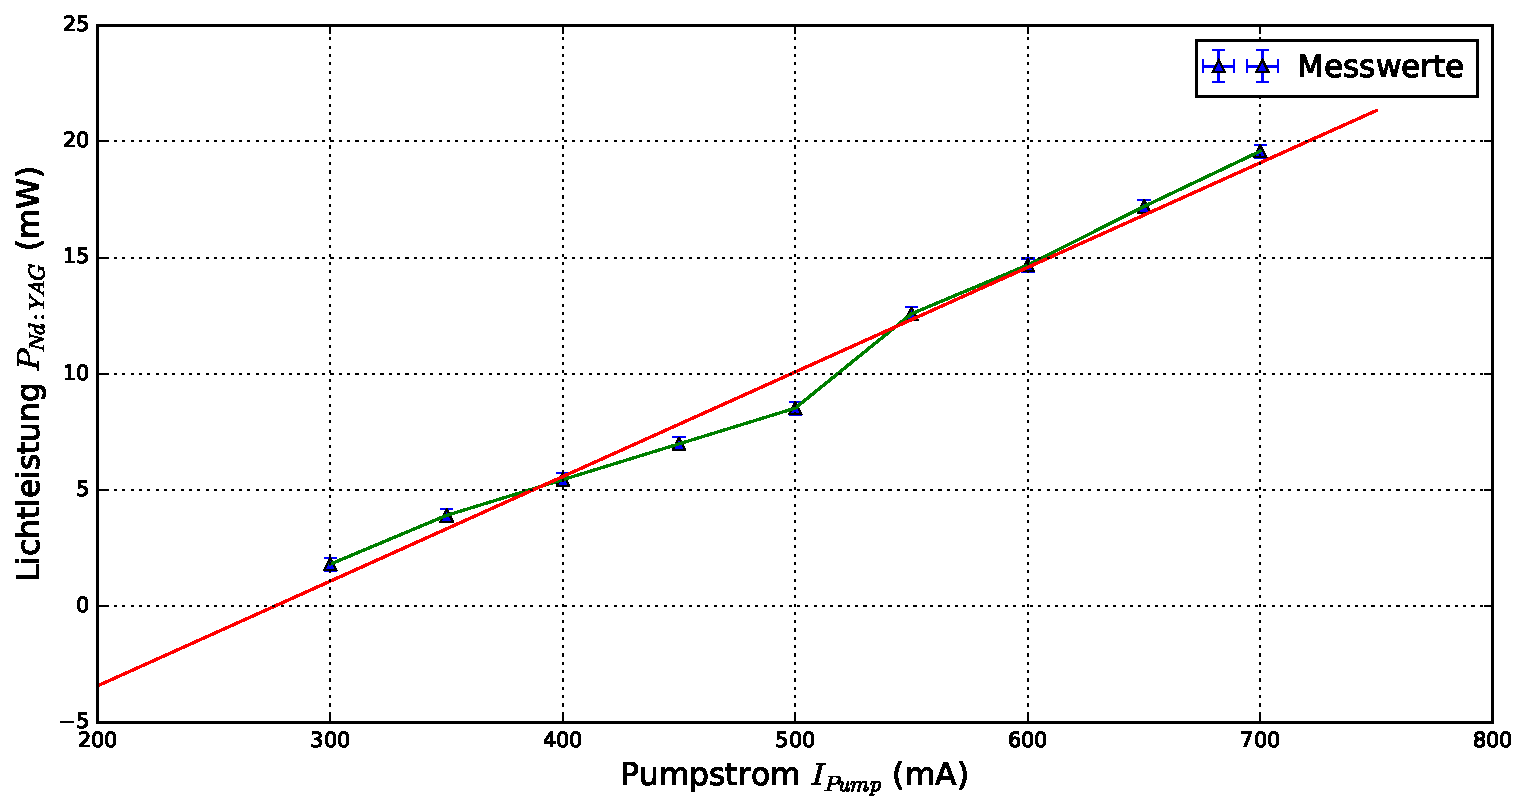
\includegraphics[width=\textwidth]{graphics/kenn_ndyag_PS.pdf}
  	\label{kenyag}
   	\end{minipage}
\caption{Kennlinie des Nd:YAG-Lasers mit Ausgleichsgerade}	
\end{figure}
Ein linearer Fit an die Daten ergab folgende Werte:
\begin{align}
m&= (0,045\pm 0,002)\,\si{\frac{mW}{mA}}\\
b&= (-12,4\pm 1,3)\,\si{mW}
\end{align}
womit der nötige Pumpstrom zu $I_{Schwelle}=(275,56\pm 28,92)\,\si{mA}$ bestimmt werden konnte. Die Differenz zum Schwellenstrom des Halbleiterlasers beträgt $\Delta I_{Schwelle}\approx 73\,\si{mA}$, da eine gwisse Pumpleistung von Nöten ist um im Nd:YAG-Kristall die Besetzungsinversion zu gewährleisten. In Abbildung \ref{kenyag2} ist die gemessene Lichtleistung des Nd:YAG Systems in Abhängigkeit der Pumpleistung der Halbleiterdiode aufgetragen. Dabei wurde der Pumpstrom und dessen Fehler mittels Gleichung \ref{kd} in eine Pumpleistung umgerechnet.
\begin{figure}[H]
\centering
   	\begin{minipage}[b]{0.85\textwidth}
   	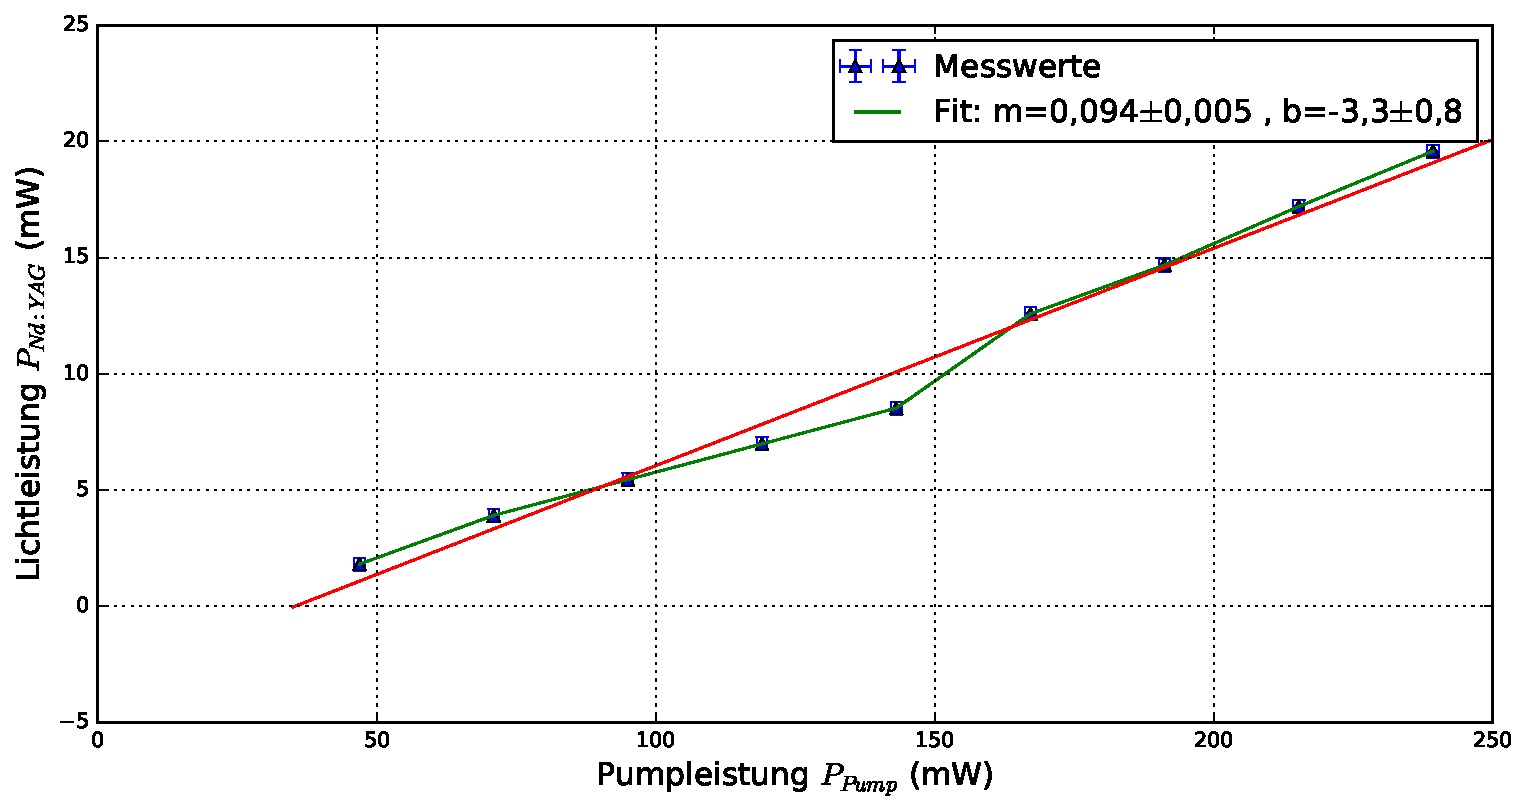
\includegraphics[width=\textwidth]{graphics/kenn_ndyag_pl.pdf}
  	\label{kenyag2}
   	\end{minipage}
\caption{Lichtleistungs-Pumpleistungskennlinie des Nd:YAG}	
\end{figure}
Für den linearen Fit ergaben sich:
\begin{align}
m=& 0,094 \pm 0,005\\
b=& -3,3 \pm 0,8
\end{align}\\
Über diese Darstellung lässt sich direkt die minimal nötige Pumpleistung $P_{Schwelle}=35,11\pm 8,71\,\si{mW} $ berechnen. Diese Lichtleistung muss minimal vom Halbleiterlaser geleistet werden, damit im Nd:YAG-Kristall Lasertätigkeit angeregt werden kann.
\pagebreak

Durch die Betrachtung der Kennlinien und des Schwellstromes/der Schwellleistung des Nd:YAG-Systems konnten die wichtigsten Charakteristika bereits herausgearbeitet werden. Im nächsten Schritt soll nun die Effizienz betrachtet werden.
Zunächst betrachten wir den Quantenwirkungsgrad $\epsilon=\frac{E_{\lambda_{Nd:YAG}}}{E_{\lambda_{Diode}}}$ welche sich mithilfe von $E_{\lambda}=\frac{hc}{\lambda}$ schreiben lässt als $\epsilon=\frac{\lambda_{Diode}}{\lambda_{Nd:YAG}}=0,76$. Es wird also theoretisch ca. $76\%$ der Pumplichtleistung in Laserlichtleistung der Wellenlänge $\lambda=1064\,\si{nm}$ umgewandelt. Betrachten wir nun noch die tatsächliche totale Leistungseffizienz des Systems $\eta_{P}=\frac{P_{Nd:YAG}}{P_{Pump}}$, welche in \ref{toleist} aufgetragen ist. Erkennbar ist, dass diese für immer größer werdende Pumpleistungen gegen $\eta_{P}\approx 9,4\%$ strebt.
Aus den Messwerten ergibt sich eine maximale Leistungseffizienz von $\eta_{max}=(8,2\pm 1,2)\%$.
\begin{figure}[H]
\centering
   	\begin{minipage}[b]{0.85\textwidth}
   	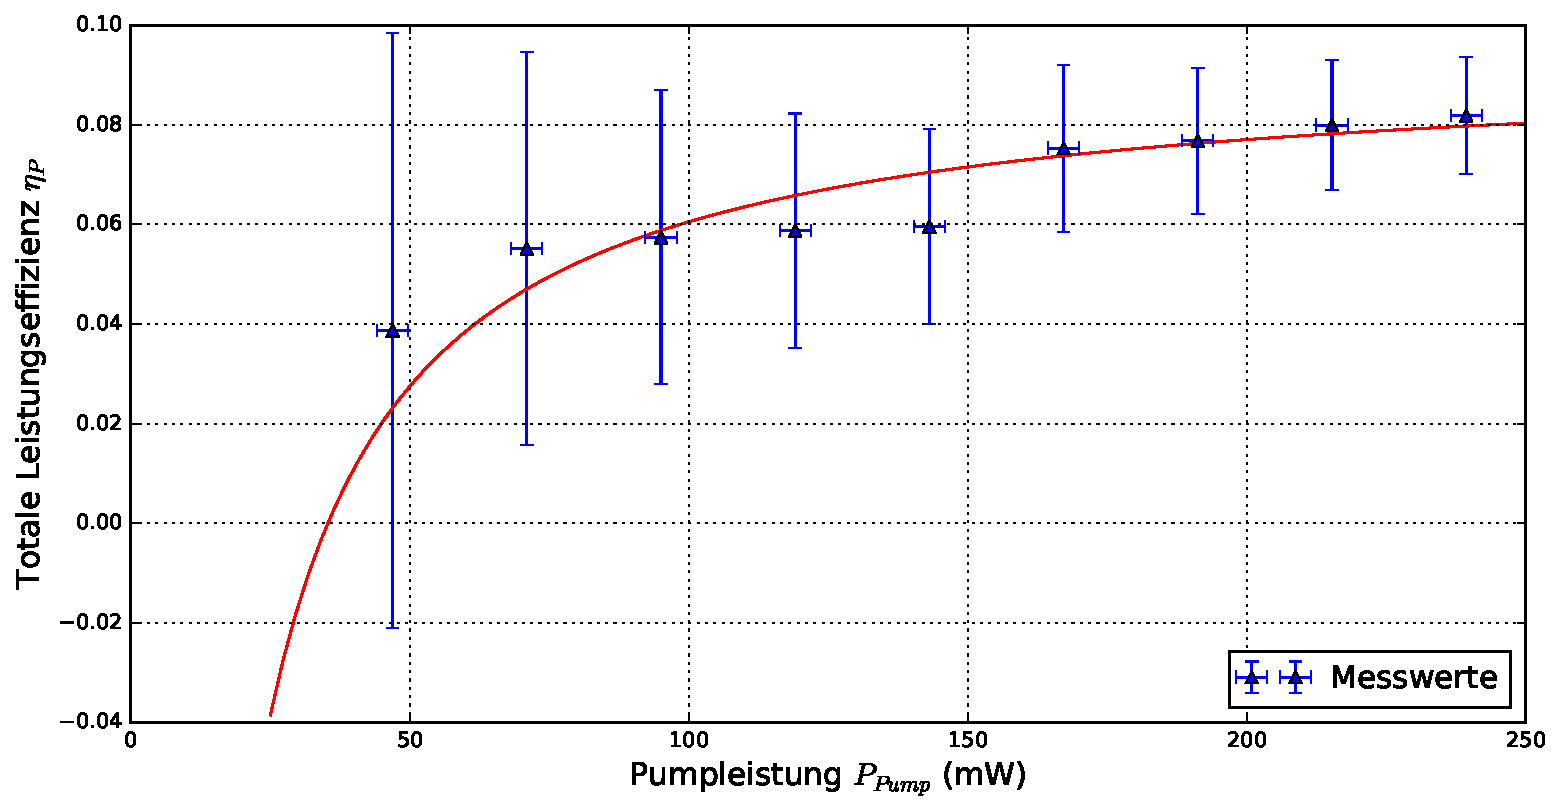
\includegraphics[width=\textwidth]{graphics/tot_leisteff.pdf}
  	\label{toleist}
   	\end{minipage}
\caption{Totale Leistungseffizienz des gesamten Systems}	
\end{figure}
Die Diskrepanz zwischen dem theoretischen Wert und der reellen Effizienz wird durch viele Faktoren beeinflusst. Zum einen ist die erfolgte die Einstellung des optischen Resonators anhand von vier Stellschrauben an Spiegel- und Kristallhalterung und wurde per Augenmaß vorgenommen. Durch eine genauere Justage sind höhere Effizienzgrade erreichbar, würden jedoch zeitlich und aufwandstechnisch den Rahmen des FP sprengen. Des Weiteren scheinen die Komponenten altersbedingt an Effizienz zu verlieren, wie der Vergleich mit den vorhandenen Daten vorheriger Versuchsteilnehmer zeigt. Noch ein Faktor der die Effizienz mindert ist das anregen höherer transversaler Moden. Idealer Weise hätte sowohl der Pumpstrahl als auch der Nd:YAG-Strahl ein transversales Gaußprofil, welches jedoch bei Betrachtung des Strahls mit einer Reflektorkarte nicht der Fall war. Statt nur einem kreisförmigen Punkt gab es zusätzlich noch mehrere Nebenpunktem, die auch durch weitere Justage zwar minimiert werden konnten, sich jedoch nicht ganz verhindern ließen. Auch durch diesen Effekt geht Lichtleistung "`verloren"'.
\pagebreak
\section{Frequenzverdopplung}
Zur Untersuchung der Frequenzverdopplung am KTP-Kristall werden zunächst die Lichtleistung des frequenzverdoppelten Anteils $P_{532\,\text{nm}}$ bei 532 nm und die Lichtleistung des Anteils bei 1064 nm $P_{1064\,\text{nm}}$ als Funktion des Pumpstroms aufgetragen. Um den Einfluss des Umgebungslichts zu untersuchen werden die Nd:YAG-Laserschwelle und die Halbleiterlaserschwelle eingetragen. Zur Messung der unterschiedlichen Kennlinien wurden verschiedene Filter verwendet. Für den Anteil bei 532 nm ergibt sich der in Abbildung \ref{a_4.4_1} dargestellte Verlauf.
\begin{figure}[H]
\centering
   	\begin{minipage}[b]{0.85\textwidth}
   	\includegraphics[width=\textwidth]{graphics/kennP532.pdf}
  	\label{a_4.4_1}
   	\end{minipage}
\caption{Leistung des frequenzverdoppelten Anteils in Abhängigkeit vom Pumpstrom}	
\end{figure}
Man erhält eine quadratische Abhängigkeit der Lichtleistung $P_{532\,\text{nm}}$ von dem Pumpstrom $I_{\text{Pump}}$. Man erhält als gefitteten Verlauf eine Parabel der Form
\begin{align*}
P_{532\,\text{nm}}(I_{\text{Pump}})= a(I_{\text{Pump}}+b)^2+c
\qquad\text{mit}\qquad
a&=(2,3 \pm 0,2)\cdot 10^{-6}\,\frac{\si{mW}}{\si{mA}}\\
b&=(348 \pm 16)  \,\si{mA}\\
c&=(2,1\pm0,5)\cdot 10^{-2} \,\si{mW}.
\end{align*}
Man kann erkennen, dass sowohl nicht bis zur Nd:YAG-Laserschwelle, als auch nicht bis zur Halbleiter-Laserschwelle gemessen wurde. Unter 300 mA wurden keine weiteren Werte aufgenommen, da sich der Photostrom nicht mehr änderte. Zudem waren die Schwankungen im Photostrom zu groß, um sinnvoll Messwerte aufnehmen zu können. Man erkennt, dass die gefitette Funktion bei etwa 350 mA ihr Minimum hat, sodass man davon ausgehen kann, dass dort der Untergrund überwiegt. Um im folgenden den Photostrom $P_U$, der durch Umgebungslicht verursacht wird zu vernachlässigen, werden die Messwerte für die Lichtleistung bei 532 nm um  $P_U=(0,021\pm0,005)$ mW nach unten korrigiert.\\
\pagebreak 

Für den Anteil bei 1064 nm ergibt sich der in Abbildung \ref{a_4.4_2} dargestellte Verlauf.
\begin{figure}[H]
\centering
   	\begin{minipage}[b]{0.85\textwidth}
   	\includegraphics[width=\textwidth]{graphics/kennP1064.pdf}
  	\label{a_4.4_2}
   	\end{minipage}
\caption{Leistung des nicht frequenzverdoppelten Anteils in Abhängigkeit vom Pumpstrom}	
\end{figure}
Die Leistung des Anteils bei 1064 nm ist linear von dem Pumpstrom $I_{\text{Pump}}$ abhängig. Man erhält den Zusammenhang
\begin{align*}
P_{1064\,\text{nm}}(I_{\text{Pump}})=m\cdot I_{\text{Pump}}+b \qquad \text{mit} \qquad
m&=(0,018\pm0,003)\,\frac{\si{mW}}{\si{mA}}\\
b&=(-5,5\pm1,3) \,\si{mW}.
\end{align*}
Man erkennt, dass sowohl nicht bis zur Nd:YAG-Laserschwelle, als auch nicht bis zur Halbleiter-Laserschwelle gemessen wurde. Aufgrund des Einbaus des KTP-Kristalls in den Bereich des Laserresonators und anschließender Neujustierung, hat sich die Nd:YAG-Laserschwelle womöglich verschoben. Zudem konnten aufgrund von zu großen Schwankungen des Photostroms unterhalb von 300 mA keine sinnvollen Werte aufgenommen werden. Da der Untergrund wesentlich kleiner als die Messwerte für die Lichtleistung bei 1064 nm ist, muss dieser nicht weiter betrachtet werden. \\

Um die Konversionseffizienz der Frequenzverdopplung am KTP-Kristall zu untersuchen wird zunächst die Lichtleistung $P_{532\,\text{nm}}$ des Anteils bei 532 nm gegen die Fundamentalleistung $P_{532\,\text{nm}+1064\,\text{nm}}$, die genähert wird als die Summe der gemessenen Leistungen des frequenzverdoppelten und des fundamentalen Lichtes, dargestellt. Die Werte der frequenzverdoppelten Leistung wurden dabei, wie zuvor erläutert nach unten korrigiert. Der gemessene Zusammenhang ist in Abbildung \ref{a_4.4_3} zu sehen.
\begin{figure}[H]
\centering
   	\begin{minipage}[b]{0.85\textwidth}
   	\includegraphics[width=\textwidth]{graphics/kennP1064532.pdf}
  	\label{a_4.4_3}
   	\end{minipage}
\caption{Leistung des frequenzverdoppelten Anteils in Abhängigkeit von der Fundaentalleistung}	
\end{figure}
Die Lichtleistung des frequenzverdoppelten Anteils hängt quadratisch von der Fundamentalleistung ab. Die quadratische Abhängigkeit ist über  
\begin{align*}
P_{532\,\text{nm}}(P_{532\,\text{nm}+1064\,\text{nm}})=a\cdot P^2_{532\,\text{nm}+1064\,\text{nm}} \qquad \text{mit} \qquad
a&=(0,0055\pm0,0003)\,\frac{\si{mW}}{(\si{mA})^2}\\
\end{align*}
gegeben.
\begin{figure}[H]
\centering
   	\begin{minipage}[b]{0.85\textwidth}
   	\includegraphics[width=\textwidth]{graphics/konveffi.pdf}
  	\label{a_4.4_4}
   	\end{minipage}
\caption{Konversionseffizienz in Abhängigkeit von der Fundamentalleistung}	
\end{figure}
\pagebreak
Die Konversionseffizienz $\upgamma_{\text{SHG}}$ ist durch
\begin{align*}
\upgamma_{\text{SHG}}=\frac{P_{532\,\text{nm}}}{P_{532\,\text{nm}+1064\,\text{nm}}}
\end{align*}
definiert.
Betrachtet man die zuvor bestimmte Abhängigkeit, so erhält man
\begin{align*}
\upgamma_{\text{SHG}}=\frac{P_{532\,\text{nm}}}{P_{532\,\text{nm}+1064\,\text{nm}}}\sim\frac{P^2_{532\,\text{nm}+1064\,\text{nm}}}{P_{532\,\text{nm}+1064\,\text{nm}}}=P_{532\,\text{nm}+1064\,\text{nm}},
\end{align*}
sodass man einen linearen Zusammenhang zwischen der Konversionseffizienz undder Fundamentalleistung erwartet. Der gemessene Zusammenhang ist in Abbildung \ref{a_4.4_4} dargestellt. 
Der erwartete lineare Zusammenhang ist zu erkennen. Wie erwartet erhält man 
\begin{align*}
\upgamma_{\text{SHG}}(P_{532\,\text{nm}+1064\,\text{nm}})=a\cdot P_{532\,\text{nm}+1064\,\text{nm}} \qquad \text{mit} \qquad
a&=(0,0055\pm0,0003)\,\frac{\si{mW}}{\si{mA}}.
\end{align*}
Die maximal erreichte gemessene Konversionseffizienz beträgt $\upgamma_{\text{SHG,max}}=0,041\pm0,003$, also etwa 4\%. Will man die Konversionseffizienz erhöhen, so kann man, wenn möglich, auf höhere Leistungen zurückgreifen. Die Frequenzverdopplung hängt stark von der Intensität der Pumpstrahlung ab und kann somit bei höheren Intensitäten besser erreicht werden. Zudem kann der Kristall über die Einstellung des Auftreffwinkels des Pumplasers so justiert werden, das die Phasenanpassung bestmöglich erfüllt ist. In dem verwendeten Versuchsaufbau konnte der Winkel nicht eingestellt werden. Um eine wesentlich höhere Effizienz zu erreichen, kann der Kristall anstatt in den Laserresonator in einem eigenen Resonator platziert werden.
\section{Vergleich mit einem kommerziellen Laserpointer}
Nachdem im Verlauf des Versuches ein grüner Laser der Wellenlänge $\lambda =532\,\si{nm}$ aufgebaut und charakterisiert wurde, soll nun der Vergleich zu einem Laserpointer, welcher auf dem gleichen Prinzip beruht, gezogen werden. Hierfür wurde zunächst die Photodiode sowie die Halterung für die Filter in den Strahlengang des Pointers montiert und dann der Photostrom sowohl mit eingebautem RG1000 als auch BG39 Filter gemessen. Des Weiteren wurde bei ausgeschaltetem Pointer der Untergrund vermessen.
Zunächst ist zu bemerken, dass sich der Photostrom bei eingebautem RG1000 Filter, welcher eine hohe Transmission für die Fundamentale $\lambda_{Fund.}=1064\,\si{nm}$ aufweist, nicht ändert, während der Pumpstrom erhöht bzw. verringert wird. Der gemessene Photostrom deckt sich außerdem mit der Höhe des gemessenen Untergrundstromes, woraus zu schließen ist, dass keine Messbare Leistung im Bereich der Wellenlänge der Fundamentalen den Laserpointer verlässt. Dies ist auch notwendig, da die Strahlung im Infraroten Bereich liegt, also nicht mit bloßem Auge sichtbar ist und somit den Lidschlussreflex nicht auslösen kann. Bei schlecht gebauten Pointern kann es dazu kommen, dass zwar die eigentliche Laserleistung im Bereich der gewollten Wellenlänge begrenzt ist, doch signifikant mehr Leistung durch die Fundamentale ausgestrahlt wird, was gesundheitliche Folgen nach sich ziehen kann.\\
Für den Laserpointer wurden folgende Messwerte bestimmt:
\begin{align}
I_{Photo}&=0,21\,\si{mA}\\
I_{Pump}&=199,6\,\si{mA}\\
V&=2,88\,\si{V}
\end{align}
Hieraus ergeben sich für die Lichtleistung unter Berücksichtigung der Transmission $T=0,71$ und der spektralen Empfindlichkeit der Photodiode von $\alpha =0,28\,\si{mA/mW}$ bei $\lambda =532\,\si{nm}$ 
\begin{equation}
P_{Pointer}=\frac{I_{Photo}}{T\cdot\alpha}=\frac{0,21\,\si{mA}}{0,71\cdot 0,28\,\si{mA/mW}}=(1,06\pm 0,02) \,\si{mW}.
\end{equation}
Bei einer elektrischen Leitung von $P_{Pump}=I_{Pump}\cdot V=199,6\,\si{mA}\cdot 2,88\,\si{V}=574,85\,\si{mW}$ ergibt sich damit eine Effizienz von $\eta=\frac{P_{Pointer}}{P_{Pump}}=(0,184\pm 0,003) \%$. Vergleicht man dies mit dem im Versuch aufgebauten Lasersystem mit einer Effizienz von $\eta=\frac{P_{Photo}}{P_{Pump}}=0,023\pm0,001 \%$, erkennt man das die Effizienz des Laserpointers ungefähr achtmal größer ist, als die des aufgebauten Systems. Dies liegt unter anderem an der händischen Justage des optischen Resonators sowie an der Grundsätzlichen Bauweise der Systeme. Im Versuch hätte eine höhere Effizienz dadurch erzielt werden können, dass der KTP-Kristall ebenfalls in einen eigenen optischen Resonator gepackt wird. Des Weiteren ist zu Beachten, dass alle im Versuch verwendeten Komponenten schon eine Längere Zeit in Verwendung sind und gerade die beiden Kristalle scheinbar einem Alterungsprozess unterliegen der die Güte und damit die Effizienz beeinflusst. Dies wurde im Gespräch mit dem Betreuer besprochen und in bei allen Prozessen beachtet.

\chapter{Fazit}
Im Verlauf des Versuches konnte erfolgreich ein frequenzverdoppeltes Nd:YAG-Laser-System mit einer gewünschten Wellenlänge von $\lambda=532\,\si{nm}$ aufgebaut, vermessen und mit einem herkömmlichen grünen Laserpointer des gleichen Prinzips verglichen werden. Der Aufbau wurde Komponentenweise vorgenommen und jede Komponente für sich näher untersucht.\\
Zunächst wurde die für das optische Pumpen des Systems zuständige Halbleiter-Laserdiode betrachtet. Da Laserdioden eine gewisse Durchstimmbarkeit in ihrer Wellenlänge aufweisen wurde zunächst mittels einer Absorptionsmessung bei maximalem Pumpstrom die optimale Temperatur ermittelt, um den Kristall bei $\lambda_{Pump}=808,4\,\si{nm}$ zu pumpen. Es ergab sich das Tupel $(I,T)=(700\,\si{mA},20\,\si{^{\circ}C})$, welches im nächsten Schritt als Startpunkt zur Bestimmung der Arbeitsgeraden diente. Um den Kristall verlässlich bei der vorgesehenen Wellenlänge und unterschiedlichen Strömen pumpen zu können, wurde eben diese Arbeitsgerade aufgenommen und der lineare Fit an die Daten diente im Laufe des Versuches dazu die Temperatur so dem Pumpstrom anzupassen, dass effizientes Pumpen gewährleistet war.
Im Anschluss wurde die Kennlinie, also die Lichtleistung der Laserdiode in Abhängigkeit des Pumpstromes durch eine Messung bestimmt. Mittels eines linearen Fits an die vorhandenen Messdaten konnte der Schwellstrom zu $I_{Schwelle}=(202,44\pm 0,80)\,\si{mA}$ bestimmt werden. Um eine weiter charakteristische Größe dieser Laserdiode zu betrachten, wurde die differentielle Quanteneffizienz, also das Verhältnis von gepumpten Elektronen zu entstandenen Laserphotonen, zu $\eta=0,314 \pm 0,001$ bestimmt. Dies bedeutet, dass nur knapp ein Drittel der gepumpten Elektronen zur Lasertätigkeit der Diode beitragen.\\
Nachdem die Laserdiode ausreichend charakterisiert wurde, konnte das nächste Bauteil dem Strahlengang hinzugefügt werden: der Nd:YAG-Kristall. Zunächst wurde der aus eine sphärischen Spiegel und der verspiegelten Rückseite des Kristalls bestehende optische Resonator auf ein Maximum im Photostrom geeicht und dann eine Messreihe zur Bestimmung der Kennlinie aufgenommen. Mittels dieser Daten konnte sowohl die Strom- als auch die Pumpleistungskennlinie ermittelst werden. Durch lineare Fits an die Daten wurde der Schwellstrom zu $I_{Schwelle}=(275,56\pm 28,92)\,\si{mA}$ und die Schwellleistung zu $P_{Schwelle}=(35,11\pm 8,71)\,\si{mW}$ bestimmt werden. Diese zeigen, dass bereits eine beträchtliche Lichtleistung (verglichen mit handelsüblichen Laserpointern) mit der Diode gepumpt werden muss, damit es im Kristall zu Lasertätigkeit kommt.
Durch Auftragen von $\frac{P_{Nd:YAG}}{P_{Pump}}$ konnte die Leistungseffizienz und deren Grenze berechnet werden. Aus den Messpunkten ergibt sich eine maximale Leistungseffizienz von $\eta_{max}=(8,2\pm 1,2)\%$, für beliebig große Pumpleistungen strebt die Lichtleistung des Nd:YAG gegen $\eta_{Grenze}\approx (9,4\pm 0,5)\%$. Im Gegensatz zu diesen knapp unter 10\% Leistungseffizienz liegt die theoretische Quanteneffizienz des Systems bei $\epsilon\approx 76\%$. Die Diskrepanz ist unter anderem durch Alterungsprozesse der Kristalle/Diode und dadurch bedingt, dass nur knapp 60\% der Pumpleistung durch Nd:YAG-Kristall in die gewünschte Wellenlänge von $\lambda=1064\,\si{nm}$ umgesetzt wird.\\
Der Laser bei 1064 nm konnte erfolgreich frequenzverdopplet werden, sodass ein sichtbarer Laserstrahl mit 532 nm erzeugt wurde. Die Lichtleistung hängt quadratisch von der Fundamentalleistung des Lasers, der für die Frequenzverdopplung verwendet wird ab. Zudem konnte gezeigt werden, dass ein linearer Zusammenhang zwischen der Fundamentalleistung und der Konversionseffizienz besteht. Die maximal erreichte gemessene Konversionseffizienz beträgt $\upgamma_{\text{SHG,max}}=0,041\pm0,003$, also etwa 4\%. Normalerweise liegt die erwartete Konversionseffizienz für das verwendete System bei etwa 10\%. Die schlechte Effizienz begründet sich vermutlich auf dem Alter des Kristalls beziehungsweise auf einer schlechten Justage des Resonators. In guten Lasersystemen, in denen der Kristall innerhalb eines eigenen Resonators platziert wird, können Konversionseffizienzen von bis zu 60\% erreicht werden.

\chapter{Messdaten}
Bestimmung der relativen Absorption. Messintervall $\delta T=2\,\si{°C}$, Fehler des Pumpstromes $\Delta I_{Pump}=2\,\si{mA}$, Fehler Temperatur $\Delta T=0,1\,\si{°C}$ Fehler Photostrom $\Delta I_{Photo}=0,2\,\si{mA}$ dieser muss jedoch noch der Skala entsprechend umgerechnet werden. Für diese Messung gilt: $30\,\si{Einheiten}$ auf der Anzeige des Multimeters entsprechen einem Photostrom von $6\,\si{mA}$.
\begin{table}[H]
\renewcommand*{\arraystretch}{1.2}
\centering
\begin{tabular}{|c|c|c|}
\hline 
T in °C & $I_{MK}$ in mA (Skala) & $I_{OK}$ in mA (Skala)\\
\hline 
10 & 7,9 & 18,0 \\ 
\hline 
12 & 4,2 & 18,0 \\ 
\hline 
14 & 3,6 & 17,9 \\ 
\hline 
16 & 3,3 & 18,0 \\ 
\hline 
18 & 3,1 & 18,1 \\ 
\hline
20 & 1,3 & 18,0 \\ 
\hline
22 & 2,1 & 17,9 \\ 
\hline
24 & 4,2 & 17,5? \\ 
\hline
26 & 6,9 & 17,9 \\ 
\hline
28 & 7,4 & 17,8 \\ 
\hline
30 & 6,6 & 17,3 \\ 
\hline
32 & 4,6 & 17,4 \\ 
\hline
34 & 4,5 & 17,2 \\ 
\hline
36 & 6,9 & 17,1 \\ 
\hline
38 & 8,5 & 17,0 \\ 
\hline
40 & 10,2 & 17,1 \\ 
\hline
\end{tabular} 
\caption{Photostrom vor Umrechnung mit und ohne Nd:YAG Kristall in Abhängigkeit der Temperatur}\label{relabs}
\end{table}

Messdaten zur Arbeitsgeraden der Laserdiode. Fehler der Temperatur $\Delta T=0,2\,\si{°C}$, Fehler des Pumpstromes $\Delta I_{Pump}=1\,\si{mA}$

\begin{table}[H]
\renewcommand*{\arraystretch}{1.2}
\centering
\begin{tabular}{|c|c|}
\hline 
$I_{Pump}$ in mA & T in °C\\
\hline 
700 & 19,8  \\ 
\hline 
675 & 20,0  \\ 
\hline 
650 & 20,2  \\ 
\hline 
625 & 20,3  \\ 
\hline 
600 & 20,5  \\ 
\hline
575 & 20,2 \\ 
\hline
550 & 21,1 \\ 
\hline
\end{tabular} 
\caption{Wertepaare der Arbeitsgeraden für $\lambda =808,4\,\si{nm}$}\label{arbger}
\end{table}

\newpage

Messdaten zur Kennlinie der Laserdiode.Es gelten die gleichen Fehler wie bisher für Pump- und Photostrom, sowie erneut die Umrechnung resultierend aus der Skala des Multimeters: $30\,\si{Einheiten}$ auf der Anzeige des Multimeters entsprechen einem Photostrom von $6\,\si{mA}$. Die beiden letzten Messwerte wurden auf einer um eine Größenordnung kleineren Skala aufgenommen und auf die vorherige umgerechnet.
\begin{table}[H]
\renewcommand*{\arraystretch}{1.2}
\centering
\begin{tabular}{|c|c|}
\hline 
$I_{Pump}$ in mA & $I_{Photo}$ in mA (Skala)\\
\hline 
700 & 16,8  \\ 
\hline 
650 & 15,3  \\ 
\hline 
600 & 13,8  \\ 
\hline 
550 & 12,1  \\ 
\hline 
500 & 10,4  \\ 
\hline
450 & 8,7 \\ 
\hline
400 & 6,5 \\ 
\hline
350 & 4,9 \\ 
\hline
300 & 3,1 \\ 
\hline
250 & 1,69 \\ 
\hline
200 & 0,06 \\ 
\hline
\end{tabular} 
\caption{Wertepaare zur Bestimmung der Kennlinie der Laserdiode}\label{kennd}
\end{table}

Messdaten zur Kennlinie des Nd:YAG Festkörperlasers. Fehler und Skala wie bisher.
\begin{table}[H]
\renewcommand*{\arraystretch}{1.2}
\centering
\begin{tabular}{|c|c|}
\hline 
$I_{Pump}$ in mA & $I_{Photo}$ in mA (Skala)\\
\hline 
700 & 14,0  \\ 
\hline 
650 & 12,3  \\ 
\hline 
600 & 10,5  \\ 
\hline 
550 & 9,0  \\ 
\hline 
500 & 6,1  \\ 
\hline
450 & 5,0 \\ 
\hline
400 & 3,9 \\ 
\hline
350 & 2,8 \\ 
\hline
300 & 1,2 \\ 
\hline
\end{tabular} 
\caption{Wertepaare zur Bestimmung der Kennlinie des Nd:YAG Lasers}\label{kennND}
\end{table}
\newpage
Messdaten zum Frequenzverdoppelten Laserlicht bei $\lambda =532\,\si{nm}$. Die Fehler bleiben gleich, jedoch gilt nun, dass $30\,\si{Einheiten}$ auf der Skala einem Photostrom von $0,6\,\si{mA}$ entsprechen.
Ab einem Pumpstron von $I_{Pump}=500\,\si{mA}$ wurde auf die Skala eine Größenordnung tiefer gewechselt und die gemessenen Werte auf die vorherige Skala angepasst und eingetragen (Filter: BG39).
\begin{table}[H]
\renewcommand*{\arraystretch}{1.2}
\centering
\begin{tabular}{|c|c|}
\hline 
$I_{Pump}$ in mA & $I_{Photo}$ in mA (Skala)\\
\hline 
700 & 3,2  \\ 
\hline 
650 & 2,3  \\ 
\hline 
600 & 1,45  \\ 
\hline 
550 & 1,1  \\ 
\hline 
500 & 0,92  \\ 
\hline
450 & 0,45 \\ 
\hline
400 & 0,37 \\ 
\hline
350 & 0,2 \\ 
\hline
300 & 0,2 \\ 
\hline
\end{tabular} 
\caption{Wertepaare zur Bestimmung der Kennlinie des KTP-Lasers}\label{kennktp}
\end{table}

Messdaten zur Bestimmung der restlichen Fundamentalleistung nach dem KTP-Kristall. Es gelten die gleichen Fehler für den Photo- und Pumpstrom wie bisher und $30\,\si{Einheiten}$ auf der Anzeige des Multimeters entsprechen einem Photostrom von $6\,\si{mA}$ (Filter:RG1000).
\begin{table}[H]
\renewcommand*{\arraystretch}{1.2}
\centering
\begin{tabular}{|c|c|}
\hline 
$I_{Pump}$ in mA & $I_{Photo}$ in mA (Skala)\\
\hline 
700 & 5,0  \\ 
\hline 
650 & 4,2  \\ 
\hline 
600 & 3,6  \\ 
\hline 
550 & 3,0  \\ 
\hline 
500 & 2,5  \\ 
\hline
450 & 1,33 \\ 
\hline
400 & 0,85 \\ 
\hline
350 & 0,5 \\ 
\hline
300 & 0,15 \\ 
\hline
\end{tabular} 
\caption{Wertepaare zur Bestimmung der restlichen Fundamentalleistung}\label{restfund}
\end{table}



		

\renewcommand{\bibname}{Literatur}
\begin{thebibliography}{0}
\bibitem {prot1} Protokoll zum Versuch 4.4: Holographie, Tatjana Beynsberger und Dominik Pfeiffer 
\bibitem {anl} Anleitung zum Versuch 4.6, Version 1.6 (06.06.2013)
\bibitem {laser} Laser, F.K. Kneubühl und M.W. Sigrist, Teubner Verlag (Literaturmappe)
\bibitem {laser2} Anleitung zum Versuch 8 Nd:YAG-Laser, RTHW Aachen, Stand 12.03.2012
\bibitem {laser3} \url{www.laserschneiden-marktplatz.de/lasertypen/ndyag-laser} (Zugriff: 09.05.2017)
\bibitem {6} Robert W. Boyd: Nonlinear Optics. Elsevier Ltd, Oxford, 3. edition, 2008.
\bibitem {7} Literaturmappe im Anhang der Versuchsanleitung zum Versuch Hong-Ou-Mandel Effekt, TU Darmstadt
\bibitem {8} Hecht, Eugene: Optics, 4. Edition, 12 August 2001
\end{thebibliography} 	



\end{document} 